\documentclass[aspectratio=1610]{beamer}
\setbeamersize{text margin left=7mm,text margin right=5mm}
\usefonttheme[onlymath]{serif}
\usetheme{default}
\usefonttheme{professionalfonts}
%\setbeamertemplate{navigation symbols}{} 
\beamertemplatenavigationsymbolsempty
\addtobeamertemplate{navigation symbols}{}{
    \usebeamerfont{footline}
    \usebeamercolor[fg]{footline}
    %\hspace{1em}
    \footnotesize\insertframenumber\,%/\inserttotalframenumber
}

% cSpell:disable
\definecolor{rcomment}{rgb}{0.3, 0.3, 0.3}  % darkgrey
\definecolor{rred}{rgb}{0.7,0.2,0.2}        % red
\definecolor{rblue}{rgb}{0.2,0.2,0.7}       % blue (blended blue of beamer)
\definecolor{rpurple}{rgb}{0.45, 0.0, 0.9}  % violett
\definecolor{rpink}{rgb}{0.8, 0.0, 0.4}     % pink
\definecolor{rgreen}{rgb}{0.1, 0.5, 0.1}    % darkgreen
\definecolor{rorange}{rgb}{0.8, 0.4,0}      % orange
\definecolor{rblack}{rgb}{0, 0, 0}          % black
\definecolor{deeptuerkis}{rgb}{0, 0.5, 0.5} % Türkis
\definecolor{darkgreen}{rgb}{0,0.5,0}
\definecolor{blendedblue}{rgb}{0.2,0.2,0.7}
\newcommand{\important}[1]{{\color{green!60!black}#1}}

% \documentclass{beamer}
% \mode<presentation> {
%   \usetheme{Singapore}
%   \setbeamertemplate{navigation symbols}{}
%   \setbeamertemplate{footline}[frame number]
% }

\usepackage[utf8]{inputenc}
\usepackage{caption}
\usepackage{nicefrac}
\usepackage{varwidth}
\usepackage{amsmath}
\usepackage{hyperref}
\usepackage{color}
\usepackage{xcolor}
\usepackage[linesnumbered, ruled, noend]{algorithm2e}
\usepackage{appendixnumberbeamer}
\usepackage{booktabs}
\usepackage{multirow}
\usepackage{multimedia}


\usepackage{natbib}
% \usepackage[backend=bibtex,style=authoryear-comp]{biblatex}
% \bibliography{bibliography}

\usepackage[draft,nomargin,inline]{fixme}  % add final for disabling remarks
\fxsetface{inline}{\itshape}
\fxsetface{env}{\itshape}
%\fxuselayouts{margin}
%\fxuselayouts{inline}
\fxusetheme{color}

\usepackage{tikz}
\usepackage{pgfplots}
\usetikzlibrary{calc, decorations.markings}
\tikzset{vertex/.style={circle, draw=black}}
\tikzset{tr/.style={draw=white, fill=white, sloped}}
\tikzset{del/.style={draw=red, text=red}}
\tikzset{layer/.style={rectangle, draw=black, minimum width=1.5cm, minimum height=0.75cm}}
\tikzset{plus/.style={
  circle, draw=black, minimum width=0.3cm, inner sep=0cm, outer sep=0cm,
  path picture={
    \draw[black] (path picture bounding box.south) -- (path picture bounding box.north)
                 (path picture bounding box.west) -- (path picture bounding box.east);
  }
}}
\tikzset{buswidth/.style={decoration={
  markings,
  mark=at position 0.5 with {\node[font=\footnotesize] {/};\node[below=3pt] {\tiny #1};}
}, postaction={decorate}}}

\pgfplotsset{compat=1.18}


\newcommand{\tmax}{\ensuremath{t^\max}}
\newcommand{\plim}{\ensuremath{p^\lim}}
\newcommand{\ILP}{\ensuremath{\mathrm{ILP}}}
\newcommand{\ppath}{\ensuremath{p^\mathrm{path}}}
\newcommand{\Tavail}{T^\mathrm{avail}}
\newcommand{\Irej}{I^\mathrm{rej}}
\newcommand{\Greedy}{\textsc{Greedy}}
\newcommand{\Markov}{\textsc{Markov}}

% \renewcommand{\thefootnote}{\fnsymbol{footnote}}
% cSpell:enable

\title{Discrete Optimization for E-Mobility}

\author{Günther R.\ Raidl}
\date{University of Canterbury, Civil and Environmental Engineering Department, NZ\\March 2, 2026}
\titlegraphic{\includegraphics[height=7mm]{graphics/logo-tuwien-informatics.png}\quad
	\includegraphics[height=7mm]{graphics/AClongColor.pdf}}

\institute[]{\normalsize Algorithms and Complexity Group, TU Wien, Austria,\\
    \texttt{raidl@ac.tuwien.ac.at}\\[1ex]
}

\logo{\includegraphics[height=15pt]{graphics/logo.pdf}\vspace{255pt}} % Logo on top right

% cSpell:disable
\definecolor{rred}{rgb}{0.7,0.2,0.2}         % red
\newcommand{\hl}[1]{\textcolor{rred}{#1}}    % highlight

\definecolor{rgreen}{rgb}{0.216,0.784,0.216} % green
\definecolor{rblue}{rgb}{0.216,0.443,0.784}  % blue
\definecolor{rorange}{rgb}{1.0,0.4,0.0}      % orange

\definecolor{orange}{RGB}{255,100,66}
\definecolor{seaborn0}{HTML}{1f77b4}
\definecolor{seaborn1}{HTML}{ff7f0e}
\definecolor{seaborn2}{HTML}{2ca02c}
\definecolor{seaborn3}{HTML}{d62728}
\definecolor{seaborn4}{HTML}{9467bd}
\definecolor{seaborn5}{HTML}{8c564b}
\definecolor{seaborn6}{HTML}{e377c2}
\definecolor{seaborn7}{HTML}{7f7f7f}
\definecolor{seaborn8}{HTML}{bcbd22}
\definecolor{seaborn9}{HTML}{17becf}

\newbool{printlegend}

\newcommand{\cumuldistr}[7]{ % Arguments: source directory, data series, width, height, x label, y label, title
  \begin{tikzpicture}
    \begin{semilogxaxis}[%
          width={#3},
          height={#4},
          title style={align=center},
          title={\large #7},
          xlabel style={at={(axis description cs:0.5,0.05)},anchor=north},
          xlabel=#5,
          ylabel style={align=center},
          ylabel=#6,
          every axis plot post/.append style={mark=none},
          every axis plot/.append style={thick},
          legend entries={GNN,Random,Sorted,Hooker},
          \ifbool{printlegend}{
            legend columns=1,
            legend pos=south east,
          }{
            legend to name=legend:cumuldistr-#1-#2,
            legend columns=-1,
          }
          ]
      \addplot+[seaborn0, solid]  table [x=#2, y=no_instances, col sep=comma, mark=none] {#1/pgdeletion_#2.csv};
      \addplot+[seaborn1, dashed] table [x=#2, y=no_instances, col sep=comma, mark=none] {#1/deletion_#2.csv};
      \addplot+[seaborn2, dashed] table [x=#2, y=no_instances, col sep=comma, mark=none] {#1/sdeletion_#2.csv};
      \addplot+[seaborn3, dashed] table [x=#2, y=no_instances, col sep=comma, mark=none] {#1/hdeletion_#2.csv};
    \end{semilogxaxis}
  \end{tikzpicture}
}
% cSpell:enable
\renewcommand{\footnotesize}{\scriptsize}

\begin{document}{}


\part{Main}

\begin{frame}
  \titlepage
\end{frame} 


\begin{frame}{Main Research Interests of G.~R.}


\medskip 
\begin{minipage}{0.45\textwidth}
  \begin{itemize}
      \item Combinatorial optimization (COP)
      \item Metaheuristics
      \item Mathematical programming
      \item Constraint programming
      \item Machine learning
      \item \important{\bf Hybrid approaches} incl.\ matheuristics, learning + classical algorithms for COP
  \end{itemize}
\end{minipage}\qquad
\begin{minipage}{0.4\textwidth}
    \structure{Application areas}
    \begin{itemize}
      \item Transport optimization
      \item Scheduling
      \item Network design
      \item Problems in bioinformatics
      \item Cutting and packing
    \end{itemize}
  \end{minipage}

  \bigskip
  \includegraphics[width=\textwidth]{graphics/AC-TU-Wien.jpg}
\end{frame}


% --------------------------------------------------------

\begin{frame}{Outline -- Recent Projects Related to E-Mobility}
	\begin{columns}[T,onlytextwidth]
		\begin{column}{0.74\textwidth}
			\begin{itemize}
				\itemsep12ex
				\item Battery Exchange Station Location Planning for E-Scooters
				\item Advanced Scheduling for Charging E-Vehicle Fleets
				\item Optimization for Electric Autonomous Dial-a-Ride Systems
				\item Conclusions
			\end{itemize}
		\end{column}
		\begin{column}{0.25\textwidth}
			\centering
			\includegraphics[width=0.9\linewidth]{graphics/scooter.jpg}\\[0.5ex]
			\includegraphics[width=0.9\linewidth]{graphics/charging.png}\\[0.5ex]
			\includegraphics[width=0.9\linewidth]{graphics/auto-vehic.png}
		\end{column}
	\end{columns}
\end{frame}


% -----------------------------------------------------
\begin{frame}[plain]
	\centering
	\vfill
	{\huge\structure{Battery Exchange Station Location Planning for E-Scooters}}
	\vfill
\end{frame}

\begin{frame}{Origins of this Project}
Former project on \structure{Public Bike Sharing Station Planning and Rebalancing}
	\begin{itemize}
	\item with City Bike Wien, NextBike, Austrian Institute of Technology
	\end{itemize} 

	\bigskip
	\begin{center}
		\includegraphics[width=0.99\textwidth]{graphics/BBSS.jpg}\\
		\citet{rainer-harbach-14}
	\end{center}

\end{frame}


\begin{frame}{Planning Battery Exchange Stations for Electric Scooters}

	Joint project with Honda Japan, Honda Research Institute Europe (2020--2024)
	
	\bigskip
	\begin{center}
		\includegraphics[width=0.7\textwidth]{graphics/bex-honda.png}
	\end{center}
\end{frame}

% \begin{frame}{A Multilevel Optimization Approach for
% 	Large Scale\\ Battery Exchange Station Location Planning}

% \citep{jatschka-23}

% \medskip
% from a joint project with Honda Japan and Honda Research Institute Europe

% \bigskip
% \begin{center}
% 	\includegraphics[width=0.6\textwidth]{graphics/Gogoro_Swapping_Station.jpg}
% \end{center}
% \end{frame}



\begin{frame}{Battery Exchange Station Location Planning (BEXLP)}
\begin{itemize}
\item \structure{Given:} 
	\begin{itemize}
		\item Potential locations for battery exchange stations
		\item Origin/Destination (O/D) pairs of expected trips \& frequency
	\end{itemize}
\item \structure{Goal:}
	\begin{itemize}
		\item Decide where to build stations with which capacities
		\item to maximize fulfilled demand while minimizing costs
	\end{itemize}
\end{itemize}

\begin{center}
	\includegraphics<1>[width=0.5\textwidth]{graphics/bex1.jpg}
	\includegraphics<2>[width=0.5\textwidth]{graphics/bex2.jpg}
	\includegraphics<3>[width=0.5\textwidth]{graphics/bex3.jpg}
	\includegraphics<4>[width=0.5\textwidth]{graphics/bex4.jpg}
	% \includegraphics[width=0.6\textwidth]{graphics/graph_second.pdf}
	% \includegraphics<2>[width=0.6\textwidth]{graphics/graph_third.pdf}
\end{center}
\end{frame}

\begin{frame}{Fulfilled Demand of O/D Pairs}
\begin{itemize}
	\item Depends on \important{detour lengths} to close stations and their \important{capacities}
\end{itemize}
\begin{center}
	%\includegraphics<1>[width=0.6\textwidth]{graphics/graph_second.pdf}
	\includegraphics[width=0.6\textwidth]{graphics/graph_third.pdf}
	\includegraphics[width=0.35\textwidth]{graphics/decay.pdf}
\end{center}
\end{frame}

\begin{frame}{Solution Approaches}
	\begin{itemize}
		\itemsep3ex
		\item \important{Mixed Integer Linear Program (MILP)}:\\ works well for small instances with \alert{few hundred} nodes and O/D pairs
		\item \important{MILP-Based Large Neighborhood Search}:\\ can handle \alert{few thousand} nodes and O/D pairs
		\item \important{Multilevel Optimization}:\\ for instances with \alert{up to 10,000 nodes and 100,000 O/D pairs}
	\end{itemize}
\end{frame}


\begin{frame}{Multilevel Optimization (MLO) by \citet{walshaw-04}}

	\begin{enumerate}
		\item \important{\bf Coarsening}: Contract graph to smaller size
		\item Repeat (1) until threshold size is reached
		\item Solve problem on the coarsest graph
		\item \important{\bf Extend and refine} solution to the next level
		\item Repeat (4) until solution to original instance is obtained
			%\item \structure{Optional:} iteratively \important{\bf recoarsen} and extend+refine 
	\end{enumerate}

	\bigskip
	\begin{center}
		\includegraphics[width=0.6\textwidth]{graphics/multilevel.jpg}\\
		%\includegraphics[width=0.6\textwidth]{graphics/mlr-gpp.png}
	\end{center}
\end{frame}

\begin{frame}{Multilevel Optimization (MLO)}
	\citep{walshaw-04}

	\bigskip
	\begin{center}
		\includegraphics[width=0.9\textwidth]{graphics/mlr-gpp.png}\\
		{\small (for graph partitioning; from \cite{walshaw-04})}
	\end{center}

\important{Solution quality strongly depends on}
\begin{itemize}
	\item coarsening strategy
	\item extension and refinement strategies
\end{itemize}
\end{frame}

\begin{frame}{Multilevel Optimization for BEXLP}
\begin{center}
	\includegraphics[scale=1.0]{graphics/MLR_example.pdf}
\end{center}
\end{frame}	

\begin{frame}{Multilevel Optimization for BEXLP}
\begin{itemize}
	\itemsep3ex
	\item Diverse clustering techniques considered
	\item MILP model used for extension/refinement
	\item Most challenging: What to take as \important{similarity measures} for
	\begin{itemize}
		\item O/D pairs to merge?
		\item for stations to merge?
	\end{itemize}
	\item Diverse similarity measures considered, ended up with Jaccard similarity
	\item In tests \important{$\approx$40--50\% better} than a reasonable construction heuristic
\end{itemize}
\end{frame}

\begin{frame}{Learning Multilevel Optimization for BEXLP}
	\citep{tomandl-24}

	\bigskip
	\begin{itemize}
		\itemsep2ex
		\item We \important{learned models to approximate the expected loss in solution quality} when
		\begin{itemize}
			\item merging two O/D pairs or 
			\item merging two stations, respectively
		\end{itemize} 
		\item Supervised learning with labels derived from
		\begin{itemize}
			\item merging pairs of nodes, solving, extension/refinement
			\item in comparison to solving original problem
		\end{itemize} 
		\item Models: multilayer perceptron with two hidden layers
		\item Diverse features derived from original nodes and merged nodes
		\item \important{Improvements of up to 1--5\% obtained}
		\item \important{Reasonable generalization to larger instances}
	\end{itemize}
\end{frame}


% -----------------------------------------------------
\begin{frame}[plain]
	\centering
	\vfill
	{\huge\structure{Advanced Scheduling for Charging E-Vehicle Fleets}}
	\vfill
\end{frame}

\begin{frame}{Charging E-Vehicle Fleets -- Basic Setting}

\begin{structure}{Given}
	\begin{itemize}
	\item Fleet of electric vehicles, for each vehicle:
	\begin{itemize}
		\item State-of-Charge (SoC)
		\item Time window for charging
		\item Required energy to be charged
	\end{itemize}
	\item Charging at common site with limited electrical power supply
	\item Photovoltaic system
	\end{itemize}
\end{structure}

\begin{structure}{Goal}
	\begin{itemize}
	\item Schedule charging of vehicles to minimize costs and maximize usage of PV
	\end{itemize}
\end{structure}

\begin{center}
	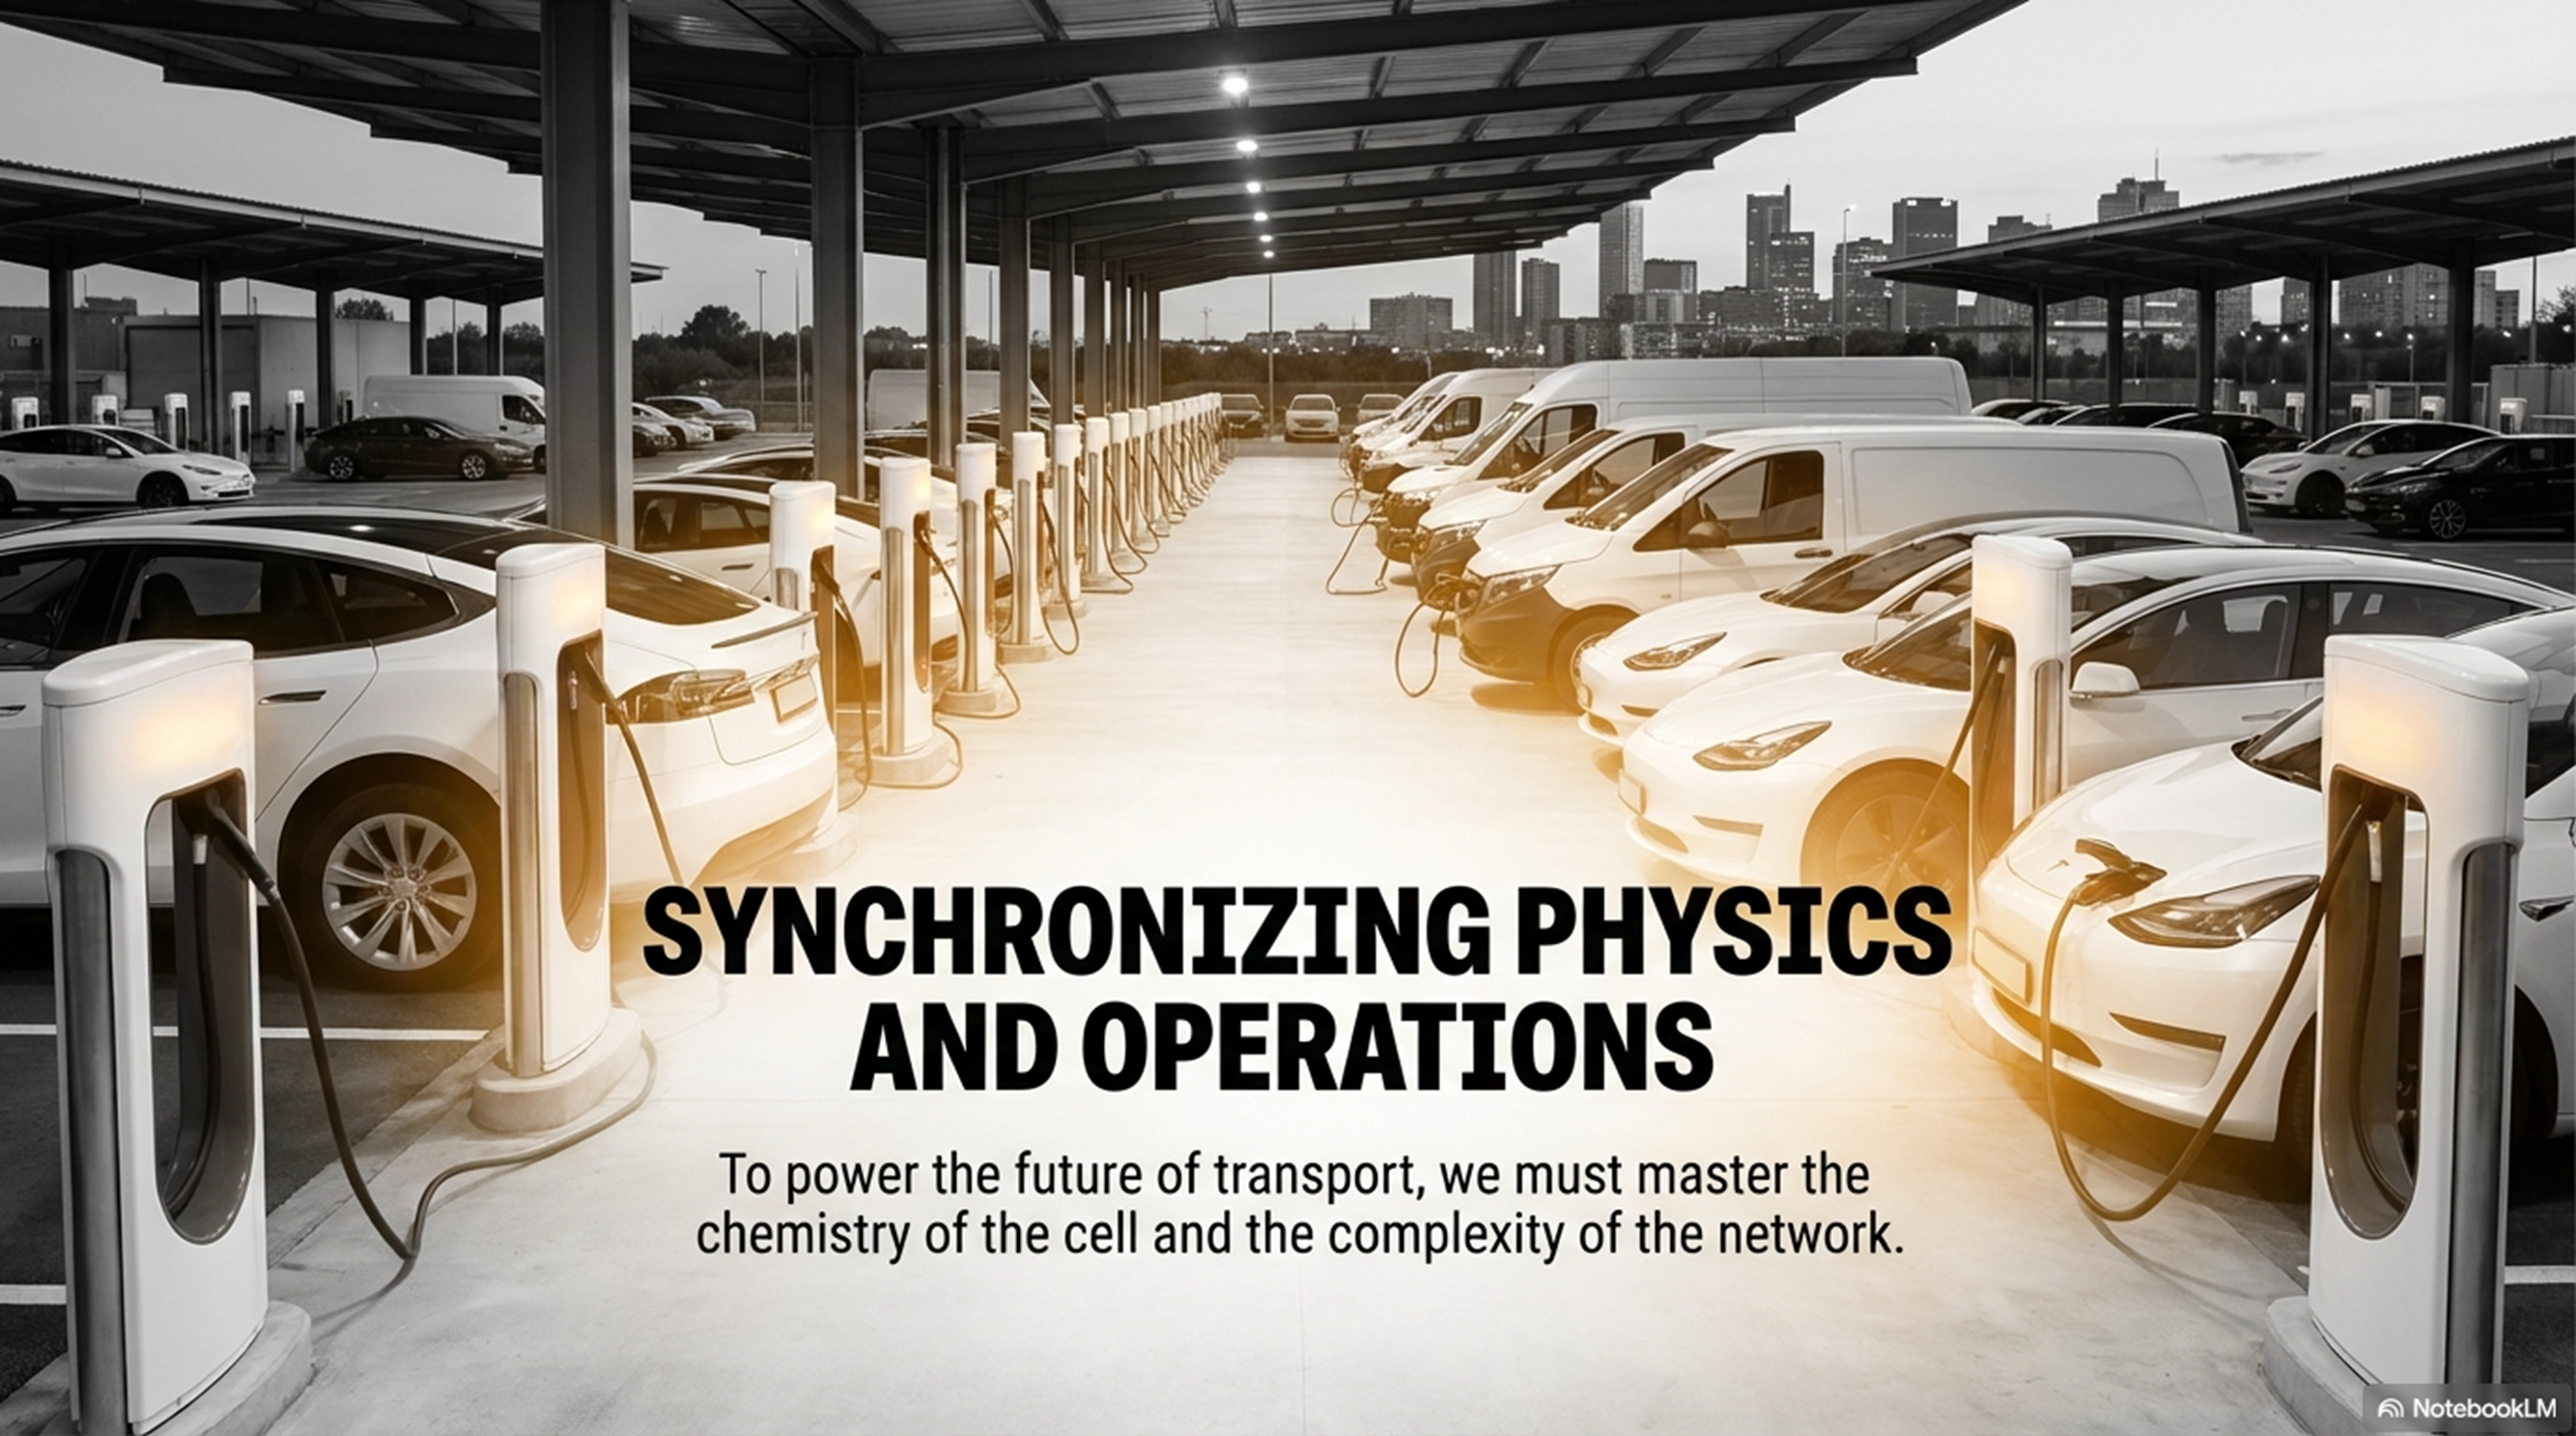
\includegraphics[width=0.5\textwidth]{graphics/fleet-charging.png}
\end{center}

%\citep{jatschka-21b,varga-22,limmer-23a,limmer-23b}
\end{frame}

\begin{frame}{Our Approaches}
\begin{itemize}
	\itemsep3ex
	\item \structure{\citet{jatschka-21b}} 
	\begin{itemize}
		\item SoC-dependent maximum charging power considered
		\item piecewise linear approximation
		\item MILP model
	\end{itemize}%
	\begin{tikzpicture}[remember picture,overlay]
		\node[anchor=north east,xshift=-6mm,yshift=-16mm,align=center] at (current page.north east) {\small Kona Hyundai\\
		\includegraphics[width=0.3\textwidth]{graphics/max-charge-power.png}};
	\end{tikzpicture}
	\item \structure{\citet{varga-22}}
	\begin{itemize}
		\item also assignment of cars to reservations considered
		\item MILP model
		\item exact Benders decomposition approach
	\end{itemize}
	\item \structure{\citet{limmer-23b}}
	\begin{itemize}
		\item for large scenarios
		\item Large Neighborhood Search (LNS) heuristic based on MILP model
	\end{itemize}
\end{itemize}

\end{frame}




% -----------------------------------------------------
\begin{frame}[plain]
	\centering
	\vfill
	{\huge\structure{The Electric Autonomous Dial-a-Ride Problem}}
	\vfill
\end{frame}


\begin{frame}
	\frametitle{The Electric Autonomous Dial-a-Ride Problem (EADARP)}

\citep{Bongiovanni:2019}

\bigskip
\structure{Given:} $n$ users with transportation requests from a pickup to a drop-off location,\\ a fleet of $m$ \important{electric autonomous} vehicles 

\medskip
\structure{Task:} Design $m$ vehicle routes serving all requests, s.t.\ the \important{total travel time and\\ the \textbf{excess ride times}} of all users are minimized and certain constraints are satisfied.
  
\begin{figure}
	\centering
	\includegraphics[scale=0.70]{graphics/darp-bss-example.jpg}
	%\caption{Example for E-DARP from \cite{Masmoudi:2018}.}
\end{figure}
	
\end{frame}

\begin{frame}
	\frametitle{Large Neighborhood Search for EADARP}

	\citep{bresich-25c}

	\bigskip
	\begin{itemize}
		\itemsep3ex
		\item \structure{Key-feature:} an efficient algorithm to insert charging station visits into routes on-the-fly
		\item \important{Leading} for benchmark instances from literature with up to \important{100 users, 8 vehicles}
	\end{itemize}
	\bigskip
 
	\only<1>{\begin{center}
		\includegraphics[width=0.45\textwidth]{graphics/lns.png}
	\end{center}}
	\pause
	\only{\structure{However:}}

	\bigskip
	\begin{itemize}
		\itemsep3ex
		\item \citet{Limmer:2023}: Simpler and faster LNS also applicable to instances with\\
		\important{few hundred vehicles, several thousand users}
		\item Our LNS only achieves \alert{few iterations within time-limit, gaps $~$10--30\%} 
		\item \important{\bf How to scale up our LNS?}
	\end{itemize}

\end{frame}

\begin{frame}
	\frametitle{Sparsening/Clustering Techniques for EADARP}

	\structure{Sparsening to $k$-nearest neighbor graph or\\ clustering into separate geographical regions}

	\pause
	\bigskip
	\alert{Does not work.} -- Why? 

	\bigskip
	Each order has
		\begin{itemize}
			\item a pickup location
			\item a dropoff location
			\item a time window
		\end{itemize}
		and orders need to be combined to tours;\\
		moreover charging not considered
	
\end{frame}

\begin{frame}
	\frametitle{Learning Heatmaps}

	\begin{itemize}
		\itemsep2ex
		\item Learn model indicating likelihood for
		\begin{itemize}
			\item pairs of orders to be served successively in same tour
			\item in (close to) optimal solutions.
		\end{itemize}
		\includegraphics[width=0.25\textwidth]{graphics/heatmap.jpg}
		\item Trained model on medium-sized instances and solutions obtained by the LNS
		\item Diverse classical ML models as well as neural networks considered;\\ \important{reasonable results obtained}
		\pause
		\item \important{More substantial improvements achieved with a \textbf{graph neural network}}
	\end{itemize}

\end{frame}


% -------------------------------------------------

\begin{frame}[plain]
	\centering
	\vfill
	{\huge\structure{Conclusions}}
	\vfill
\end{frame}

\begin{frame}
	\frametitle{Conclusions}
	\medskip
	\begin{itemize}
		\itemsep4ex
		\item Many \important{challenging optimization problems} exist in E-mobility
		\item Better solutions can have \important{dramatic impact} in energy/cost savings and user satisfaction
		\item Many optimization techniques available, but all have \important{strengths and weaknesses}
		\item We work on \important{improving/combining/tailoring algorithms} to address\\ \important{large-scale real-world problems} in better ways
	\end{itemize}
\end{frame}


\begin{frame}[allowframebreaks]
	\frametitle{References}
	%\footnotesize
	%\nocite{*} 
	% \bibliographystyle{abbrv}
	\bibliographystyle{apalike}
	\bibliography{lit.bib}
\end{frame}



\end{document}
